% Created 2019-12-30 月 20:22
% Intended LaTeX compiler: pdflatex
\documentclass[presentation,dvipdfmx,CJKbookmarks]{beamer}
\usepackage{CJKutf8}
\usepackage{atbegshi}
\AtBeginShipoutFirst{\special{pdf:tounicode UTF8-UTF16}} % for UTF-8
\usepackage[utf8]{inputenc}
\usepackage[T1]{fontenc}
\usepackage{graphicx}
\usepackage[export]{adjustbox}
\usepackage{lmodern}
\usepackage{grffile}
\usepackage{longtable}
\usepackage{wrapfig}
\usepackage{rotating}
\usepackage[normalem]{ulem}
\usepackage{amsmath}
\usepackage{textcomp}
\usepackage{amssymb}
\usepackage{capt-of}
\usepackage{hyperref}
 \usepackage{minted}
\usetheme{EastLansing}
\usecolortheme{default}
\author{Bao Haojun}
\date{2019-12-31}
\title{Programming for Fun}
\subtitle{做一个快乐编程的文艺青年\text{\includegraphics[width=1em,valign=t,raise=0.1em,natwidth=48bp,natheight=48bp]{/home/bhj/src/github/Wrench/release/emojis/weibo-new/ErHa.png}}}
\hypersetup{
 pdfauthor={Bao Haojun},
 pdftitle={Programming for Fun},
 pdfkeywords={},
 pdfsubject={},
 pdfcreator={Emacs 26.3 (Org mode 9.1.9)},
 pdflang={English}}
\begin{document}
\begin{CJK*}{UTF8}{simsun}

\maketitle
\begin{frame}{Outline}
\tableofcontents
\end{frame}

\CJKtilde

\section{Wishful Thinking(许愿式编程)}
\label{sec:orga978ccd}

\begin{frame}[fragile,label={sec:org2da35e9}]{SICP\thinspace 介绍(Structure and Interpretation of Computer Programs)}
 \pause
\begin{block}{\sout{一个小目标?先挣他一个亿?}}
\pause
\end{block}
\begin{block}{怎么定义有理数及其各种运算?}
\pause
\begin{itemize}[<+->]
\item 很简单,假设我们有\thinspace 3\thinspace 个函数:\texttt{make-有理数},\texttt{取分母},\texttt{取分子}
\item 举例:有理数乘法

\begin{minted}[]{common-lisp}
(defun 有理数乘法 (有理数a 有理数b)
  (make-有理数
   (* (取分子 有理数a) (取分子 有理数b))
   (* (取分母 有理数a) (取分母 有理数b))))
\end{minted}
\end{itemize}
\end{block}
\end{frame}

\begin{frame}[label={sec:orgc61e60b}]{Get Things Done\thinspace 工作方法}
\pause
\begin{itemize}[<+->]
\item Coders at Work\thinspace 中对\thinspace jwz\thinspace 的采访

“我就是列个单子,然后一项一项的划掉”

\begin{center}

\includegraphics[width=3cm]{./jwz.ps}
\end{center}

\item org-mode\thinspace 演示(agenda\thinspace 功能)

\begin{center}

\includegraphics[width=3cm]{./org-mode.ps}
\end{center}
\end{itemize}
\end{frame}

\begin{frame}[label={sec:orgc153370}]{Literate Programming(文艺青年的编程方法)}
\begin{itemize}[<+->]
\item Knuth\thinspace 的工作方法

\begin{center}
\includegraphics[height=3cm]{./knuth.ps}
\end{center}
\end{itemize}

\pause
\begin{itemize}
\item org-mode\thinspace 演示(knuth-mode)
\end{itemize}
\pause
\begin{itemize}
\item GTD/LP:不焦虑的秘密
\end{itemize}
\pause
\begin{itemize}
\item 盗梦空间(fence-edit-mode)
\end{itemize}
\end{frame}

\section{Abstraction}
\label{sec:orgf29cc07}

\begin{frame}[label={sec:org7a5e043}]{一本书:How to Design Programs}
\pause
\begin{block}{Abstraction(抽) \& Similarity(象)}
\pause
\end{block}
\begin{block}{Similarity \& Copying \& Problems}
\pause
\begin{itemize}
\item 有一个功能很好用,在别的地方,我也想要类似的功能(抽象 + wishing)
\end{itemize}
\pause
\end{block}
\begin{block}{Similarity \& Learning \& Oppotunities}
\end{block}
\end{frame}

\begin{frame}[fragile,label={sec:orgcffa470}]{REPL(Read、Eval、Print、Loop)}
 \begin{block}{Read}
\end{block}
\begin{block}{Eval}
\begin{itemize}
\item 注意求值的次数限制(只能求一次)
\begin{itemize}
\item 有些值求一次和求\thinspace N\thinspace 次都是一样的
\item 除此之外,不能随意求多次(如果想求多于一次,必须明确指定——比如用\thinspace eval\thinspace 函数)

\texttt{x=y; y=z; echo \$x}
\item 左值和右值有没有分别?(Tcl\thinspace 和\thinspace Perl\thinspace 的对比)
\end{itemize}
\end{itemize}
\end{block}

\begin{block}{Print}
\end{block}
\begin{block}{Loop}
\end{block}
\end{frame}

\section{Style}
\label{sec:orgaf8b985}

\begin{frame}[fragile,label={sec:orgcfe7bb1}]{编码风格(规范)与表达沟通}
 \begin{itemize}[<+->]
\item 跳过所有语言、社区、公司的编码风格
\item The Elements of Style(所有编程语言风格书致敬的对象)
\item If you don't know how to pronounce a word, say it loud!Why compound ignorance with inaudibility?
\begin{itemize}
\item -- E.B. White,The Elements of Style\thinspace 的作者之一,著有“夏洛特的网”
\item 个人而言,直接决定了我最喜欢的编程语言特性,是\thinspace shell\thinspace 的“set -e”
\item 或许我们应该学习\thinspace APUE\thinspace 的作者的做法?他把每一个常用库函数,都自己封装了一下,比如\thinspace \texttt{close(fd) -> Close(fd)},一旦发现错误返回值就退出
\end{itemize}

\begin{itemize}
\item 波尔和费曼的故事:开会之前,先找费曼聊
\end{itemize}
\end{itemize}
\end{frame}

\section{Flow}
\label{sec:org268ed36}

\begin{frame}[label={sec:org07770fa}]{}
\begin{block}{Flow\thinspace 的模型}
\begin{center}
\includegraphics[width=4cm]{./images/flow.ps}
\end{center}
\pause
\begin{itemize}[<+->]
\item 集中营里有人能活下来?
\item 截了肢的人还能觉得自己比以前还幸福?
\item “偏执于有用的细节,偏执于无用的细节,偏执于甚至不会被发现是有用还是无用的细节,这就是工匠精神”
\item “On Writing”一书作者的故事
\item Be Water My Friend -- Bruce Lee.
\end{itemize}
\end{block}
\end{frame}

\section{领导、决策与系统}
\label{sec:org5849074}

\begin{frame}[label={sec:org1474580}]{原子弹研发的保密和安全}
\begin{itemize}
\item 绝密任务,不能让纳粹知道消息
\begin{itemize}
\item 不告诉工人自己天天处理的是什么
\end{itemize}
\item 非常危险,万一超过“临界质量”的原料堆在一起,引发连锁反应。。。
\item 最后找一个上校报告,上校说,给我\thinspace 5\thinspace 分钟时间
\end{itemize}
\end{frame}

\begin{frame}[label={sec:orge6a6eec}]{关于决策系统的思考}
\begin{itemize}
\item 5\thinspace 分钟就做一个决定?
\item 决定的影响有多深远?
\begin{itemize}
\item 推荐阅读:The Fifth Discipline
\end{itemize}
\item 做决策,最关键的是什么?
\pause
\begin{itemize}
\item 承担责任
\end{itemize}
\end{itemize}
\end{frame}


\section{学习,通过编程来学习}
\label{sec:org8736c77}

\begin{frame}[label={sec:org81a9aa7}]{}
\begin{block}{man\thinspace 手册中的搜索、Text::CSV\thinspace 中的\thinspace imenu}
\end{block}
\begin{block}{info\thinspace 手册中的搜索}
\end{block}
\begin{block}{源码搜索:beagrep}
\end{block}
\begin{block}{抄书式学习(\href{https://www.zhihu.com/question/28951394}{章亦春}) => 编辑式学习 => 快捷短语}
\end{block}
\end{frame}

\section{2019\thinspace 年我的开源项目}
\label{sec:orgeb59848}
\begin{frame}[label={sec:org0f37ae5}]{2019\thinspace 年我的开源项目}
\begin{enumerate}
\item org-kungfu\thinspace 和\thinspace jkd(用\thinspace emacs\thinspace + cli\thinspace 操作\thinspace altassian\thinspace 软件)
\item cuty(个人成长辅助集中注意力软件)
\item 用\thinspace emacs\thinspace 聊钉钉
\item 简陋密码管理软件
\item 快捷短语输入(Stallman\thinspace 的故事)
\begin{itemize}
\item jira\thinspace 文档\thinspace url\thinspace 地址
\end{itemize}
\end{enumerate}
\end{frame}

\section{参考书目}
\label{sec:orga8c2dca}

\begin{frame}[label={sec:org724efe4}]{}
\begin{itemize}
\item Coders at Work
\item SICP
\item HtDP
\item The Elements of Style
\item The Fifth Discipline: The Art \& Practice of the Learning Organization
\item Flow: The Psychology of Optimal Experience
\item SURELY YOU ARE JOKING, MR. FEYNMAN!
\end{itemize}
\end{frame}
\section{Q \& A}
\label{sec:org6b51010}
\begin{frame}[label={sec:org05ed7d7}]{Q \& A}
\begin{block}{Questions\text{\includegraphics[width=1em,valign=t,raise=0.1em,natwidth=48bp,natheight=48bp]{/home/bhj/src/github/Wrench/release/emojis/qq-emojis/smiley_32.png}}}
\pause
\end{block}
\begin{block}{祝大家新年快乐!}
\pause
\end{block}
\begin{block}{记得许愿哦!}
\end{block}
\end{frame}
\end{CJK*}
\end{document}
